\documentclass[12pt, a4paper]{article}
\usepackage[utf8]{inputenc}
\usepackage[T2A]{fontenc}
\usepackage{indentfirst, setspace}
\usepackage{tabularx, multirow}
\usepackage[normalem]{ulem}
\usepackage[style=russian]{csquotes}
\usepackage[english,russian]{babel}
\usepackage{hyperref}
\usepackage{ragged2e}
\usepackage{caption}
\usepackage{wrapfig}
\usepackage{amsmath}
\usepackage{tikz}
\makeatletter
\def\@biblabel#1{#1. }
\makeatother
\captionsetup{labelsep=endash}
\usepackage{listings}
\linespread{1.3}
\lstset{
  language=C++,
  basicstyle=\ttfamily\small,
  keywordstyle=\color{blue},
  breaklines=true,
  commentstyle=\color{green},
  stringstyle=\color{red},
  extendedchars=\true,
  showstringspaces=false,
  keepspaces=true,
}

\usepackage[left=2cm,right=2cm,
    top=2cm,bottom=2cm,bindingoffset=0cm]{geometry}\begin{document}
\begin{titlepage}
     \fontsize{12}{12}\selectfont

  {\centering

   \begin{bf}

    \begin{wrapfigure}{l}{10mm}
        
\includegraphics[width=17mm]{photo_2023-12-25.jpeg}
    \end{wrapfigure}


    \noindent Министерство науки и высшего образования Российской Федерации

    \noindent Федеральное государственное бюджетное образовательное учреждение высшего образования

    \noindent \enquote{Московский государственный технический университет

     \noindent имени Н.Э. Баумана

     \noindent (национальный исследовательский университет)}

    \noindent (МГТУ им. Н.Э. Баумана)

   \end{bf}
  }

  \vspace{0.4cm}

  {\setstretch{0.1}
   \noindent\rule{\textwidth}{1mm}
   \noindent\rule{\textwidth}{0.5mm}

  }

  \fontsize{14}{21}\selectfont

  \noindent\begin{tabularx}{\textwidth}{l >{\centering\arraybackslash}X}
   ФАКУЛЬТЕТ & \flqq Фундаментальные Науки\frqq \\ \cline{2-2}

   КАФЕДРА & ФН-12 \flqq Математическое моделирование\frqq \\ \cline{2-2}
  \end{tabularx}

  \vspace{1cm}


  \begin{center}
   \begin{bf}

    \fontsize{24}{36}\selectfont
    ОТЧЕТ

    \fontsize{20}{30}\selectfont
    ПО ЛАБОРАТОРНОЙ РАБОТЕ НА ТЕМУ:

    Сжатие по Хаффману

   \end{bf}
  \end{center}

  \fontsize{14}{21}\selectfont
  \vspace{5cm}


  \noindent\begin{tabularx}{\textwidth}{ X >{\centering}p{4cm} p{1cm} c }
   Студент: & & & Мациевский И. М. \\ \cline{2-2} \cline{4-4}
   & \fontsize{10}{15}\selectfont дата, подпись & & \fontsize{10}{15}\selectfont Ф.И.О. \\
   Преподаватель: & & & Волкова Л. Л.\\ \cline{2-2} \cline{4-4}
   & \fontsize{10}{15}\selectfont дата, подпись & & \fontsize{10}{15}\selectfont Ф.И.О.
   \end{tabularx}

  \vspace{\fill}

  \begin{center}
   \it{Москва}, 2023
  \end{center}

  \thispagestyle{empty}
\end{titlepage}\newpage
\tableofcontents
\newpage
\section*{Введение}
\addcontentsline{toc}{section}{Введение}
\textbf{Цель лабораторной работы}: реализовать алгоритмы сжатия по Хаффману.

Для достижения поставленной цели требуется решить следующие \textbf{задачи}.
\begin{enumerate}
\item Описать сжатие по Хаффману.
\item Реализовать сжатие файла.
\item Реализовать возможность считывать данные из 
файла.
\item Реализовать возможность записать ответ в 
бинарный файл.
\item Провести небольшое исследование для 10 файлов с одинаковым характером 
наполнения (с увеличением размера на каждом шаге не менее, чем на 20 \%) с 
оценкой эффекта от сжатия, визуализировать результаты в виде графика.

\end{enumerate}

Согласно варианту, требуется разработать сжатие 
файла по Хаффману для нотной записи формата инструмент-темп-скорость.
\newpage
\section{Аналитическая часть}
\textbf{Сжатие по Хаффману ---} это метод сжатия 
данных, при котором используется оптимальное 
префиксное бинарное дерево, которое называется 
деревом Хаффмана. Основная идея заключается в том, чтобы присвоить 
более короткие бинарные коды (битовые последовательности) более часто 
встречающимся символам или фрагментам данных.
Процесс построения дерева Хаффмана включает следующие шаги.
\begin{enumerate}
	\item \textbf{Вычисление частот символов ---} подсчитываются частоты 
	встречаемости каждого символа или символьного фрагмента в исходных 
	данных.
	\item \textbf{Построение дерева.} Строится бинарное дерево, где 
	каждый лист представляет собой символ или фрагмент данных, а 
	расстояние от корня до листа соответствует длине кода. Чем ближе к 
	корню, тем короче код.
	\item \textbf{Присвоение кодов.} Каждому символу присваивается 
	уникальный бинарный код, который представляет собой 
	последовательность на пути от корня до листа в дереве.
	\item \textbf{Сжатие данных.} Заменяются исходные данные 
	соответствующими бинарными кодами. Более часто встречающиеся 
	символы получают более короткие коды, что обеспечивает общее 
	уменьшение объема данных.
	\item \textbf{Декодирование.} При восстановлении данных 
	используется тот же дерево Хаффмана для раскодирования бинарных 
	данных и восстановления исходных символов или фрагментов.
\end{enumerate}
\newpage
\section{Конструкторская часть}
Ниже представлены структуры и методы, реализованные в работе.
\begin{enumerate}
	\item Структура $Node$: узел дерева Хаффмана. Содержит информацию 
	об идентификаторе, частоте, а также указатели на левого и правого 
	потомков.
	\item Метод $getNode$ создает новый узел с указанным 
	идентификатором, 
	частотой и потомками.
	\item Структура $Compare$ оператор сравнения, необходимый для 
	приоритетной очереди при построении дерева Хаффмана. Он 
	используется для сравнения частот узлов. Для его работы 
	перегружается оператор $()$. Сравнивается значение $freq$ (частота) 
	для двух узлов. Если частота узла $l$ больше частоты узла $r$, то 
	метод возвращает $true$, что говорит о том, что узел $l$ имеет 
	более высокий приоритет. Иначе возвращает $false$. 
	\item $encode$ рекурсивно проходит по дереву и строит Хаффман-коды 
	для каждого узла. Код для каждого листа (конечного узла) 
	записывается в $huffmanCode$.
	\item $writeHuffmanCodesToFile$ записывает Хаффман-коды 
	(идентификаторы, частоты, длины кодов) и закодированный текст в 
	бинарный файл.
	\item $gain$ рассчитывает выигрыш от сжатия по Хаффману: в $bit1$
	хранится количество бит в исходном тексте (без сжатия), в $bit2$
	хранится количество бит в сжатом тексте после применения 
	Хаффман-кодов.\\
	$dataSize$ представляет собой размер метаданных, 
	которые записываются в бинарный файл. Для каждого идентификатора 
	записывается сам идентификатор (строка), частота ($int$) и длина 
	Хаффман-кода ($char$).\\
	$compressedSize$ представляет собой размер закодированного 
	текста после применения Хаффман-кодов.\\
	$win$ это отношение количества бит в исходном тексте 
	к общему размеру сжатых данных и метаданных.
	\item $buildHuffmanTree$ используется в построении кодов Хаффмана для
	уникальных идентификаторов (в данном случае, нот) в тексте. Ниже представлен
	алгоритм работы.
		\begin{enumerate}
			\item Проход по тексту и подсчет частоты каждого уникального 
			идентификатора (ноты).
			\item Создание приоритетной очереди для узлов дерева с учетом 
			частоты. На этом этапе каждый уникальный идентификатор (нота) 
			представляется в виде узла дерева.
			\item Используя приоритетную очередь, строится дерево Хаффмана. На 
			каждом шаге извлекаются два узла с наименьшей частотой, создается 
			новый узел с их суммарной частотой, и этот новый узел добавляется 
			обратно в приоритетную очередь. Процесс повторяется до тех пор, пока 
			в приоритетной очереди не останется только один узел - корень дерева 
			Хаффмана.
			\item Рекурсивно обходится дерево Хаффмана, начиная с корня, и 
			присваиваются уникальные коды (строки из '0' и '1') каждому узлу.\\
			Коды сохраняются в $huffmanCode$.
			\item Создается закодированный текст, при этом каждый уникальный 
			идентификатор заменяется его соответствующим кодом Хаффмана.
			\item Коды и метаданные записываются в бинарный файл 
			$Huffman_codes.bin$. В файле каждый уникальный идентификатор 
			представлен своим строковым представлением, за которым следует его 
			частота и длина кода.
			\item Выводится информация о том, во сколько раз удалось сжать 
			исходный текст с использованием алгоритма Хаффмана.
		\end{enumerate}
\end{enumerate}
\newpage
\section{Технологическая часть}
Для реализации выбран язык C++.
На листинге 1 представлена реализация программы
(Реализация~\ref{lst:label1})
\begin{lstlisting}[caption={Исходный код}, label={lst:label1}]
#include <iostream>
#include <fstream>
#include <queue>
#include <map>
#include <vector>
#include <string>

using namespace std;

struct Node {
    string id;
    int freq;
    Node* left, *right;
};

struct Compare {
    bool operator()(Node* l, Node* r) {
        return (l->freq > r->freq);
    }
};

Node* getNode(string id, int freq, Node* left, Node* right) {
    Node* node = new Node();
    node->id = id;
    node->freq = freq;
    node->left = left;
    node->right = right;
    return node;
}

void encode(Node* root, string str, map<string, string>& huffmanCode) {
    if (root == nullptr) return;
    if (!root->left && !root->right) {
        huffmanCode[root->id] = str;
    }
    encode(root->left, str + "0", huffmanCode);
    encode(root->right, str + "1", huffmanCode);
}

void writeHuffmanCodesToFile(const map<string, string>& huffmanCode, const string& encodedText, const map<string, int>& freq) {
    ofstream outputFile("/Users/ilya/Downloads/Типы и структуры данных 2 курс, 1 семестр/laba_7/laba_7/Huffman_codes.bin", ios::binary);

    if (outputFile.is_open()) {
        for (const auto& pair : huffmanCode) {
            // Записываем уникальный строковый идентификатор ноты
            outputFile.write(pair.first.c_str(), pair.first.size());
            outputFile.put('\0');  // Разделитель между идентификатором и частотой

            int frequency = freq.at(pair.first);
            outputFile.write(reinterpret_cast<const char*>(&frequency), sizeof(frequency));

            char codeLength = static_cast<char>(pair.second.length());
            outputFile.put(codeLength);
        }

        outputFile.put('\0'); // Разделитель между метаданными и закодированным текстом

        for (char ch : encodedText) {
            outputFile.put(ch);
        }

        outputFile.close();
        cout << "Данные успешно записаны в бинарный файл 'huffman_codes.bin'" << endl;
    }
    else {
        cout << "Невозможно открыть файл для записи" << endl;
    }
}

void gain(string text, const map<string, string>& huffmanCode, const map<string, int>& freq) {
    int bit_1 = text.size();
    int bit_2 = 0;

    for (const auto& pair : huffmanCode) {
        bit_2 += pair.second.size() * freq.at(pair.first) + pair.first.size() + pair.second.size();
    }

    int compressedSize = bit_2;  // размер закодированного текста в байтах
    double win = (bit_1 + 0.0) / (compressedSize);
    
    cout << "Сжатие в " << bit_1 << " байт / (" << compressedSize << " байт + " << " байт) = " << win << " раз" << endl;
}



void buildHuffmanTree(string text) {
    map<string, int> freq;
    size_t pos = 0;
    size_t nextPos = text.find('\n', pos);

    while (nextPos != string::npos) {
        string id = text.substr(pos, nextPos - pos);
        freq[id]++;
        pos = nextPos + 1;
        nextPos = text.find('\n', pos);
    }

    priority_queue<Node*, vector<Node*>, Compare> pq;

    for (const auto& pair : freq) {
        pq.push(getNode(pair.first, pair.second, nullptr, nullptr));
    }

    while (pq.size() != 1) {
        Node* left = pq.top(); pq.pop();
        Node* right = pq.top(); pq.pop();

        int sumFreq = left->freq + right->freq;
        pq.push(getNode("", sumFreq, left, right));
    }

    Node* root = pq.top();

    map<string, string> huffmanCode;
    encode(root, "", huffmanCode);

    string encodedText;
    pos = 0;
    nextPos = text.find('\n', pos);

    while (nextPos != string::npos) {
        string id = text.substr(pos, nextPos - pos);
        encodedText += huffmanCode[id];
        pos = nextPos + 1;
        nextPos = text.find('\n', pos);
    }

    cout << "Частоты идентификаторов нот: " << endl;
    for (const auto& pair : freq) {
        cout << pair.first << " : " << pair.second << endl;
    }
    cout << endl;

    cout << "Код идентификаторов нот: " << endl;
    for (const auto& pair : huffmanCode) {
        cout << pair.first << " : " << pair.second << endl;
    }
    cout << endl;

    cout << "Закодированный текст по Хаффману: " << encodedText << endl;

    writeHuffmanCodesToFile(huffmanCode, encodedText, freq);
    cout << endl;
    gain(text, huffmanCode, freq);
}

int main() {
    setlocale(0, "");
    ifstream file("/Users/ilya/Downloads/Типы и структуры данных 2 курс, 1 семестр/laba_7/input.txt");  // Замените путь на путь к вашему файлу
    string text = "";

    if (file.is_open()) {
        string line;
        while (getline(file, line)) {
            text += line + '\n';
        }
        file.close();
    }
    else {
        cout << "Невозможно открыть файл";
        return 0;
    }

    cout << "Прочитанный текст: " << endl << text << endl;
    buildHuffmanTree(text);

    return 0;
}
\end{lstlisting}
\newpage
\textbf{Примеры работы.}

Далее на рисунках 1-10 представлен результат работы программы. Размер входного 
файла с каждым тестом уменьшается на $20~\%$.
Входной файл --- уникальный строковый идентификатор ноты в формате 
инструмент-темп-скорость.  
\begin{enumerate}
	\item Входной файл --- уникальный строковый идентификатор ноты.
	Результат приведён на рис.~\ref{img:grap1}.
	\begin{figure}[h]
  		\center{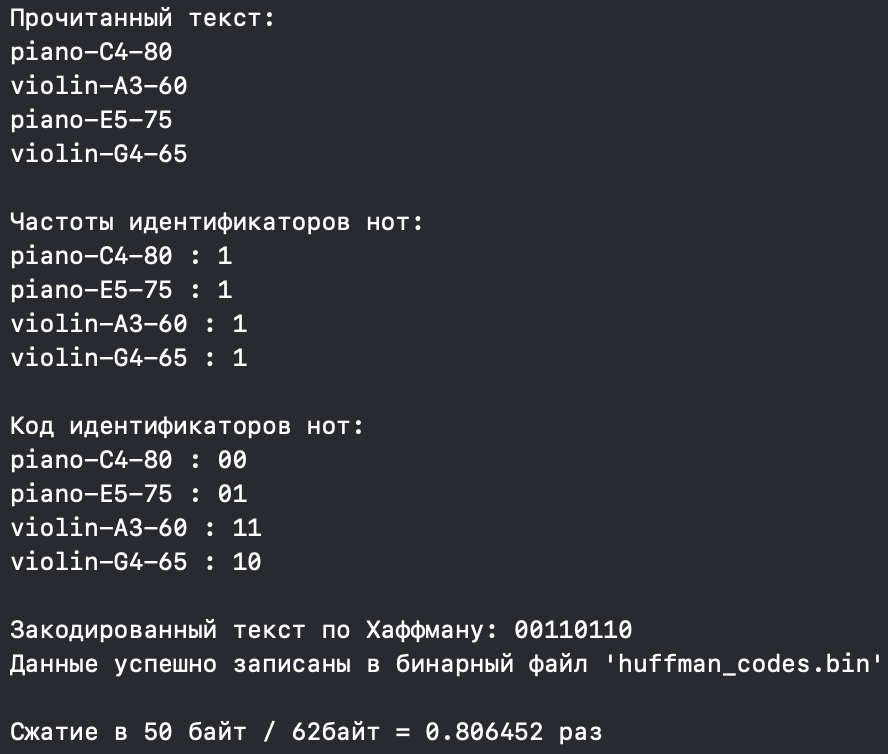
\includegraphics[scale=0.7]{ex1.png}}
  		\caption{Пример работы 1}
  		\label{img:grap1}
	\end{figure}
	\newpage
	\item Входной файл --- уникальный строковый идентификатор ноты.
	Результат приведён на рис.~\ref{img:grap2}.
	\begin{figure}[h]
  		\center{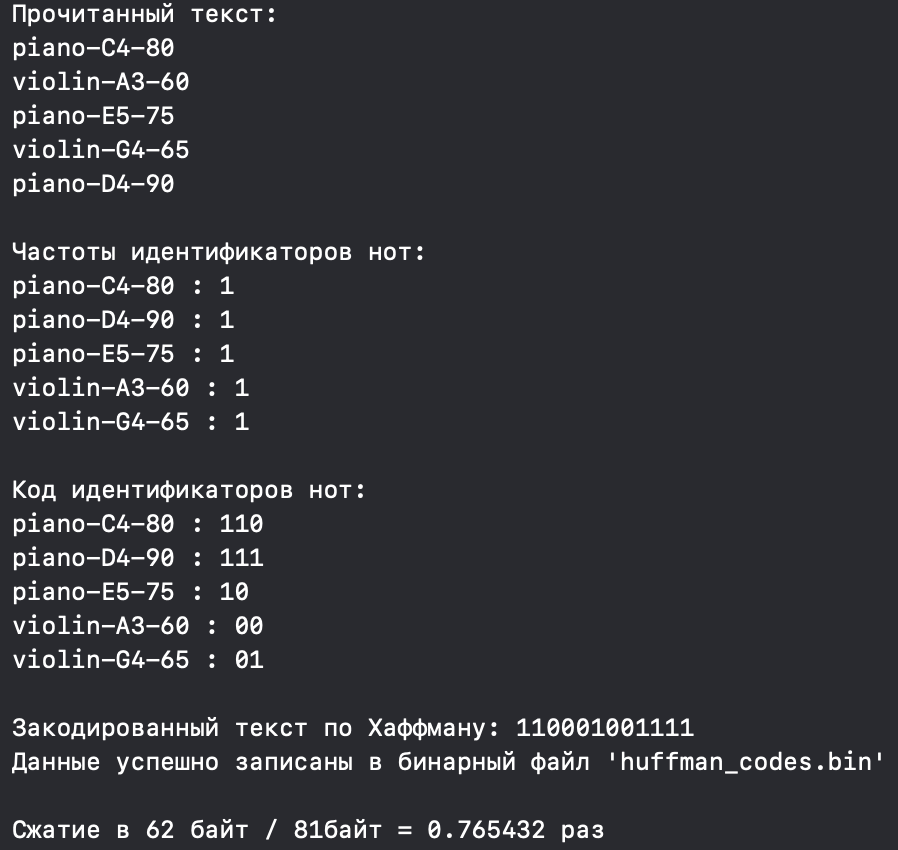
\includegraphics[scale=0.7]{ex2.png}}
  		\caption{Пример работы 2}
  		\label{img:grap2}
	\end{figure}
	\newpage
	\item Входной файл --- уникальный строковый идентификатор ноты.
	Результат приведён на рис.~\ref{img:grap3}.
	\begin{figure}[h]
  		\center{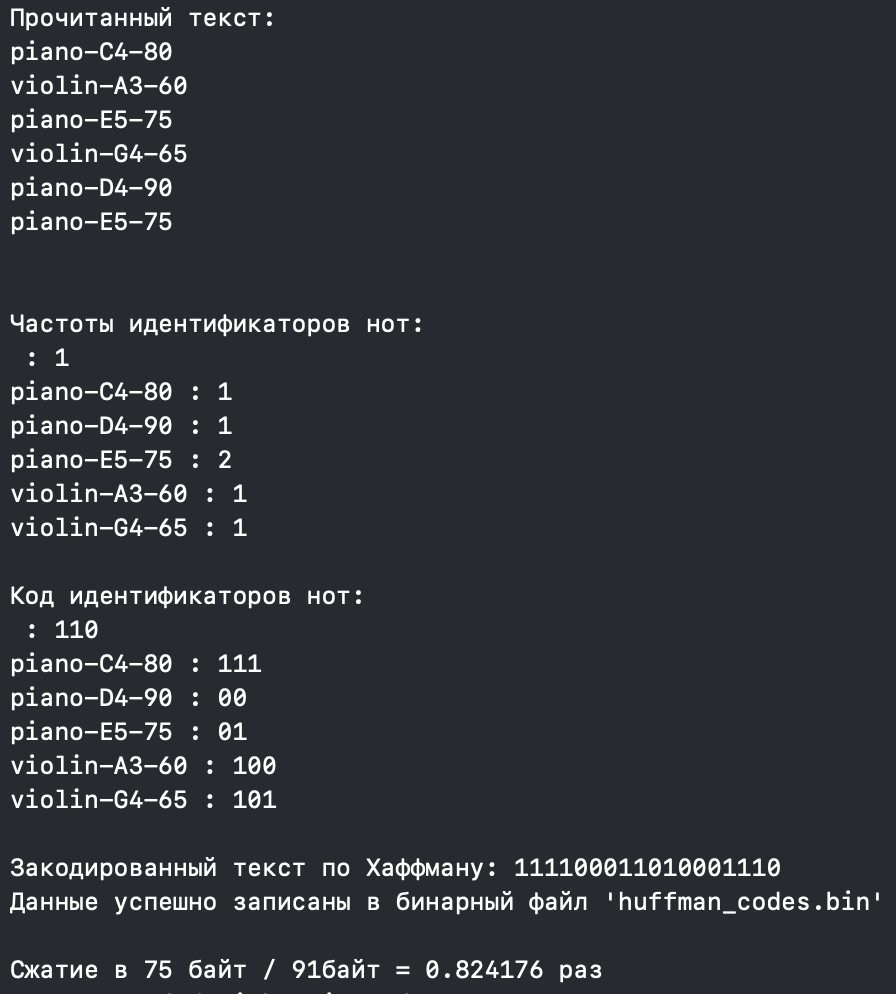
\includegraphics[scale=0.7]{ex3.png}}
  		\caption{Пример работы 3}
  		\label{img:grap3}
	\end{figure}
	\newpage
	\item Входной файл --- уникальный строковый идентификатор ноты.
	Результат приведён на рис.~\ref{img:grap4}.
	\begin{figure}[h]
  		\center{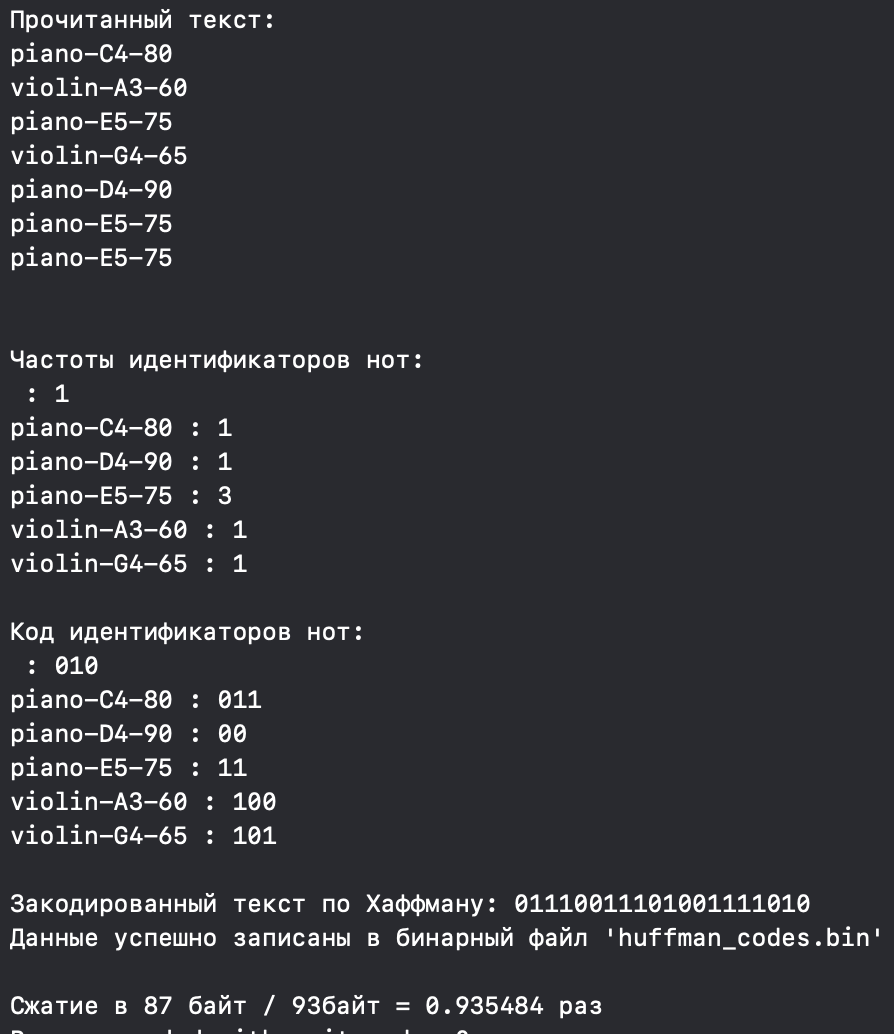
\includegraphics[scale=0.7]{ex4.png}}
  		\caption{Пример работы 4}
  		\label{img:grap4}
	\end{figure}
	\newpage
	\item Входной файл --- уникальный строковый идентификатор ноты.
	Результат приведён на рис.~\ref{img:grap5}.
	\begin{figure}[h]
  		\center{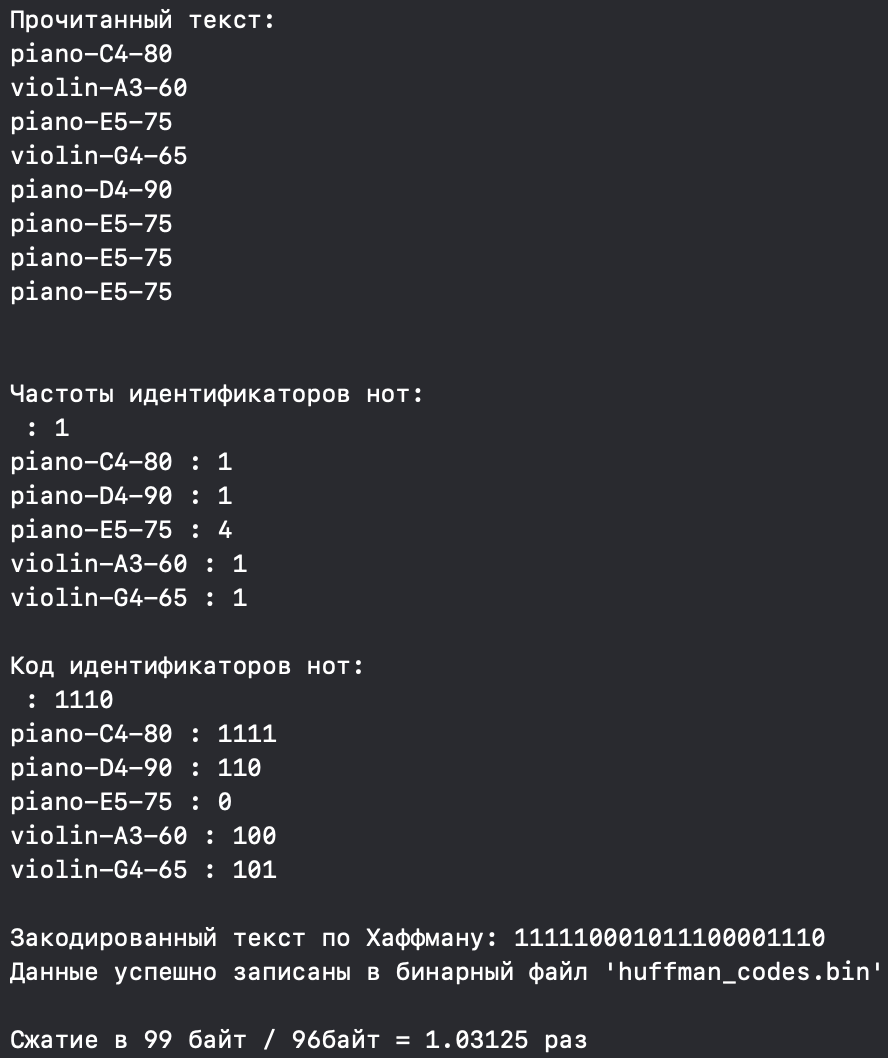
\includegraphics[scale=0.7]{ex5.png}}
  		\caption{Пример работы 5}
  		\label{img:grap5}
	\end{figure}
	\newpage
	\item Входной файл --- уникальный строковый идентификатор ноты.
	Результат приведён на рис.~\ref{img:grap6}.
	\begin{figure}[h]
  		\center{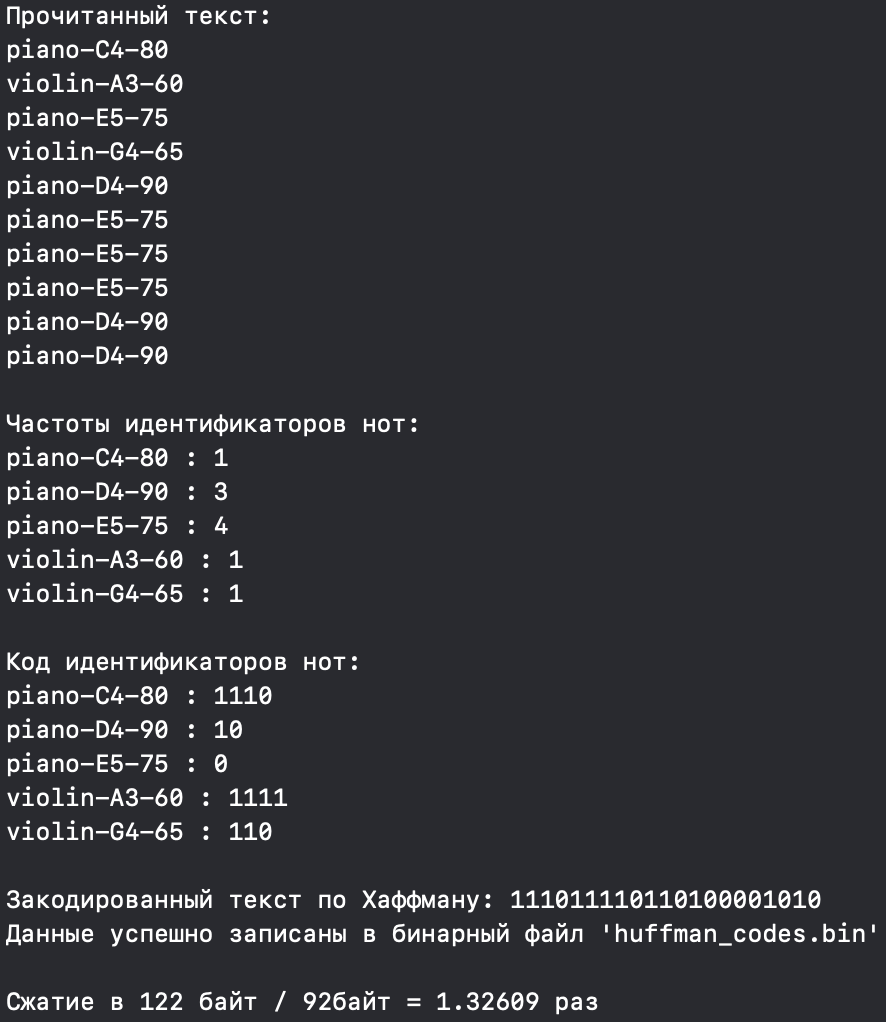
\includegraphics[scale=0.7]{ex6.png}}
  		\caption{Пример работы 6}
  		\label{img:grap6}
	\end{figure}
	\newpage
	\item Входной файл --- уникальный строковый идентификатор ноты.
	Результат приведён на рис.~\ref{img:grap7}.
	\begin{figure}[h]
  		\center{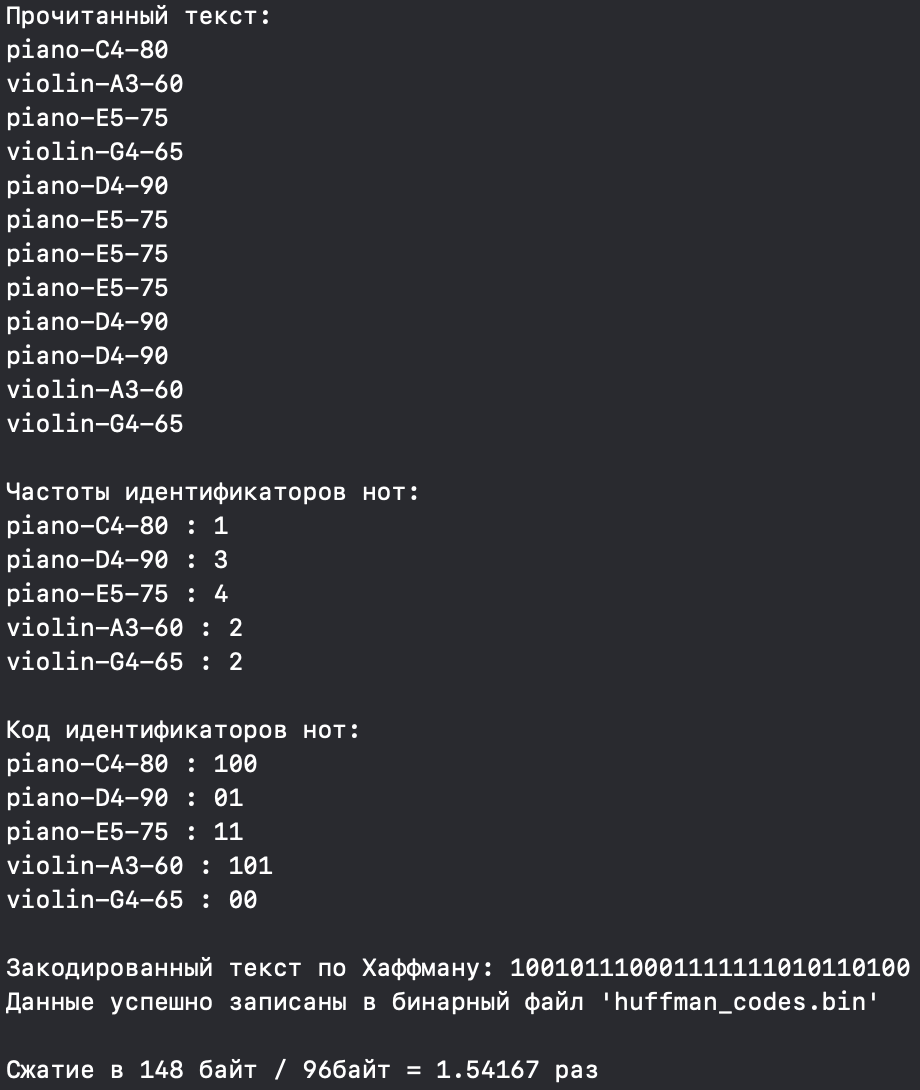
\includegraphics[scale=0.7]{ex7.png}}
  		\caption{Пример работы 7}
  		\label{img:grap7}
	\end{figure}
	\newpage
	\item Входной файл --- уникальный строковый идентификатор ноты.
	Результат приведён на рис.~\ref{img:grap8}.
	\begin{figure}[h]
  		\center{
\includegraphics[scale=0.7]{ex8.png}}
  		\caption{Пример работы 8}
  		\label{img:grap8}
	\end{figure}
	\newpage
	\item Входной файл --- уникальный строковый идентификатор ноты.
	Результат приведён на рис.~\ref{img:grap9}.
	\begin{figure}[h]
  		\center{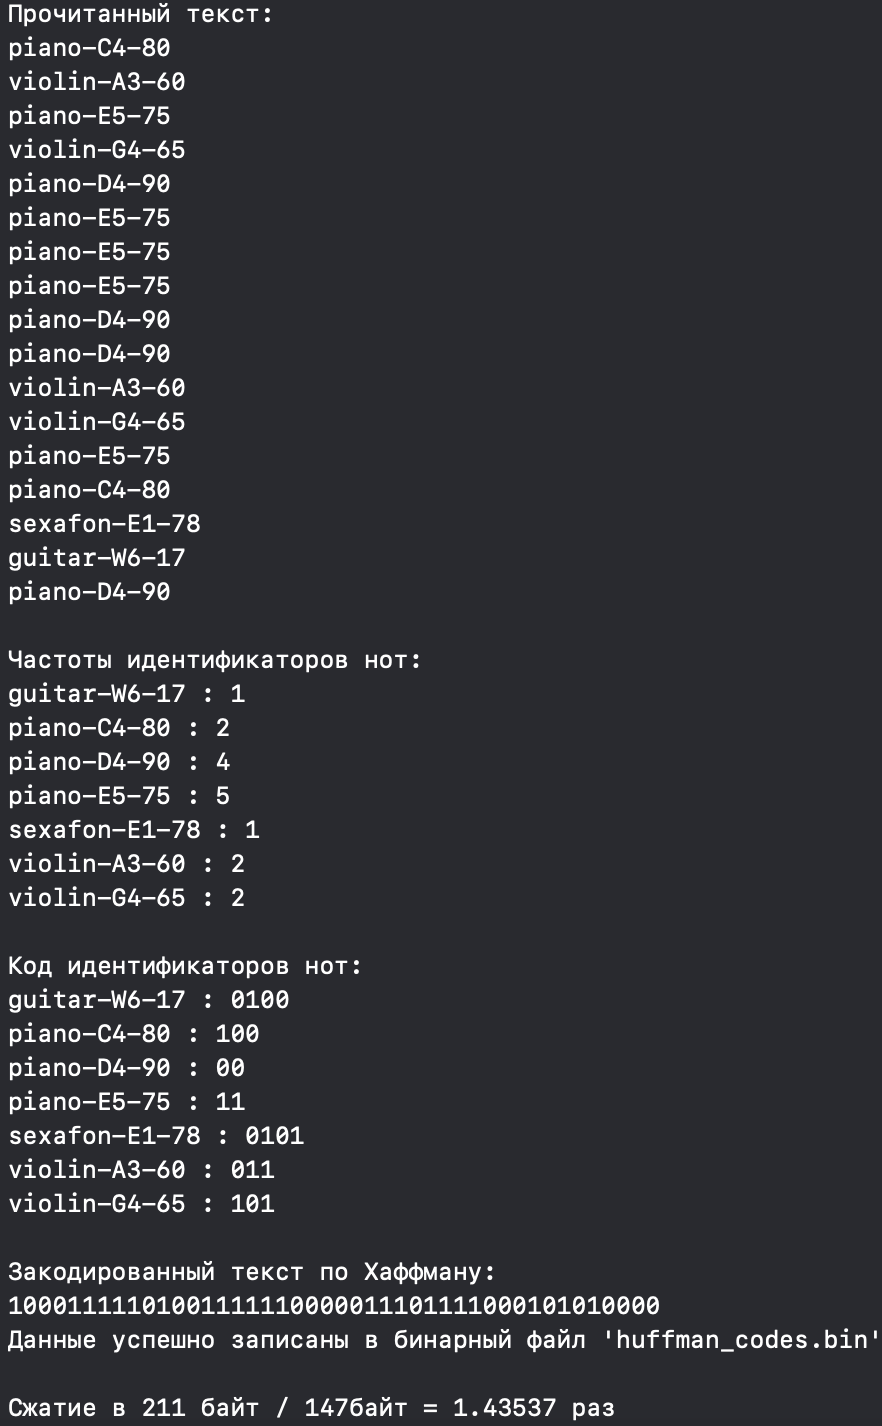
\includegraphics[scale=0.7]{ex9.png}}
  		\caption{Пример работы 9}
  		\label{img:grap9}
	\end{figure}
	\newpage
	\item Входной файл --- уникальный строковый идентификатор ноты.
	Результат приведён на рис.~\ref{img:grap10}.
	\begin{figure}[h]
  		\center{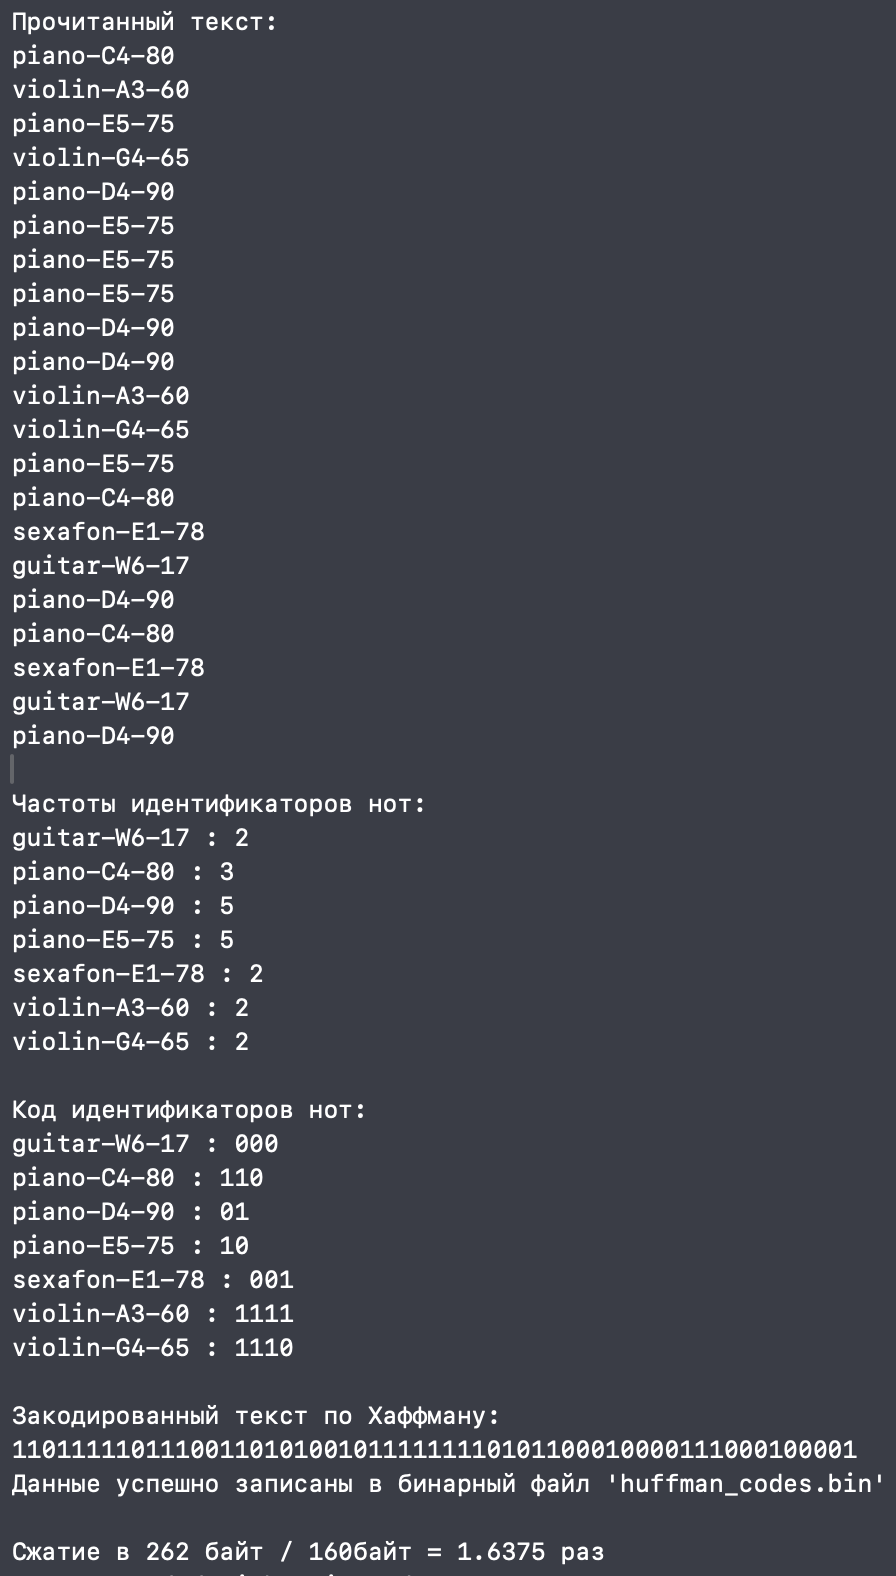
\includegraphics[scale=0.68]{ex10.png}}
  		\caption{Пример работы 10}
  		\label{img:grap10}
	\end{figure}
\end{enumerate}
\newpage
\section{Исследовательская часть}
Анализируя выполненные тесты, можно отметить, что при увеличении объема данных 
алгоритм Хаффмана становится более эффективным. Это происходит благодаря 
созданию оптимальных кодов для 
представления данных: наиболее часто встречающиеся символы кодируются более 
короткими кодами, что позволяет значительно сократить общий размер данных.

Однако нотная запись очень разнообразна, а значит есть вероятность того, 
что большое количество нот будет встречаться один раз, то есть сжатие по 
Хаффману будет невыгодно из-за того, что при данном типе сжатия хранится не
только сжатая запись, но и данные для декодирования. 

Визуализация исследования представлена на рис.~\ref{img:grap11}.
\begin{figure}[h]
  		\center{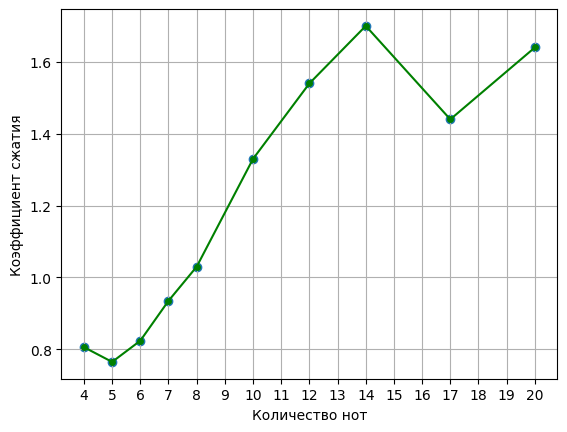
\includegraphics[scale=0.68]{graphic.png}}
  		\caption{Зависимость коэффициента сжатия от размера входых данных}
  		\label{img:grap11}
	\end{figure}

Таким образом, при увеличении объема данных сжатие по Хаффману обычно становится 
эффективнее, но для данных формата нотной записи он может быть
неэффективен как на больших, так и на маленьких типах данных.
\newpage
\section*{Заключение}
\addcontentsline{toc}{section}{Заключение}
Цель достигнута: реализованы алгоритмы сжатия по Хаффману. В результате 
были выполнены все задачи:
\begin{enumerate}
\item Описано сжатие по Хаффману.
\item Реализовано сжатие файла.
\item Реализована возможность считывать данные из 
файла.
\item Реализована возможность записать ответ в 
бинарный файл.
\item Проведено исследование для 10 файлов с одинаковым характером 
наполнения (с увеличением размера на каждом шаге не менее, чем на 20 \%) с 
оценкой эффекта от сжатия, результаты визуализированы в виде графика.
\end{enumerate}
\newpage
\begin{center}
\begin{thebibliography}{}
\addcontentsline{toc}{section}{Список используемых источников}
\bibitem{book} Котиева, Х. М. Сжатие данных без потерь. Использование алгоритма Хаффмана / Х. М. Котиева. — Текст : непосредственный // Молодой ученый. — 2020. — № 35 (325 с.).
\end{thebibliography}
\end{center}
\end{document}